\documentclass{beamer}
\usepackage[english,ngerman]{babel}
\usepackage[utf8]{inputenc}
\usepackage[T1]{fontenc}
\usepackage[autostyle,babel,german=guillemets,style=german]{csquotes}

%---------------------------------------------------------------------
% Globale Variabeln
%---------------------------------------------------------------------
\newcommand{\event}{Hochvolt Systeme}
\newcommand{\location}{Bochum}
\newcommand{\dt}{\today}
\newcommand{\x}[1]{\mathrm{#1}}  		
%---------------------------------------------------------------------

\usepackage[%
 backend=biber,%
 style=authoryear,%
 bibstyle=authoryear,%
 citestyle=authoryear,%
 natbib=false,%
 sorting=anyt,%
 sortcites=true,%
 hyperref=auto,%
 maxnames=3,%
 minnames=1,%
 refsection=subsection,%
 dashed=false%
]{biblatex}

\bibliography{bibo}
\setlength{\bibitemsep}{0.5em}

\defbibheading{bibliography}[\bibname]{%
\subsubsection*{#1}%
\markboth{#1}{#1}}

\usetheme[%
wiwi,
%nav,        		  	%% Schaltet die Navigationssymbole ein
%frutiger,				%% Ändert die Schrift in Frutiger
%mathpazo,				%% mathpazo Schrift
%mathptmx,				%% Times Schrift
colorful,    			%% Farbige Balken im infolines-Theme
%infoSub,				%% Aktiviert Infoline mit Subsections
infoline,				%% Aktiviert die Infoline über dem Frametitle
squares,     			%% Aufzaehlungspunkte rechteckig
nologo       			%% Kein Logo im Seitenhintergrund
]{FUH}

\title[Parameteridentifikation]{Ansätze zur Parameteridentifikation einer PMSM}

\author[Benjamin Ternes]%
{%
Benjamin Ternes
}

\institute{%
Hochschule Bochum\\
Fachbereich Elektrotechnik und Informatik}

\AtBeginSection[]{%
  \begin{frame}[plain] %<beamer>
    \frametitle{Agenda}
    \tableofcontents[currentsection]
     % \tableofcontents[sectionstyle=show/hide,subsectionstyle=hide/show/hide]
  \end{frame}
  % \addtocounter{framenumber}{-1}% If you don't want them to affect the slide number
}

\begin{document}

\begin{frame}[plain]
	\titlepage
\end{frame}

\begin{frame}[plain]{Autor}
Benjamin Ternes

GitHub: \url{http://github.com/benjiternes/ident.git}

\begin{itemize}
	\item VDE (Verband der Elektrotechnik Elektronik Informationstechnik e.\ V.\ ) Mitglied, Bezirk Düsseldorf	\url{http://www.vde.com/}
	\item VDI (Verein Deutscher Ingenieure) \url{https://www.vdi.de/}
	\item IEEE \url{https://www.ieee.org/index.html}
	\item Dante e.\ V.\ Mitglied~--~Deutschsprachige Anwendervereinigung TeX e.\ V.\ \url{http://www.date.de/}
\end{itemize}
\vspace{1cm}
Publikationen:\\
\fullcite{ternes2012}
\end{frame}

\begin{frame}[plain]{Agenda}
	\tableofcontents
\end{frame}

\section{Einleitung}
\begin{frame}{Allgemeines}
\begin{itemize}
\item PMSM in einer Vielzahl unterschiedlicher Anwendungen (vorallem kleinen bis mittleren Leistungen)
\item Hochdynamische Antriebsmotoren (hochdynamische Regelung)
\item Hochdynamische Regelungen benötigen die »Induktivitäten« der Maschine (abh. vom momentanen Strom)
\item Flussverkettung $\Psi$ ändert sich aufgrund von Alterungserscheinungen und Temperaturveränderungen
\item Ohmscher Ständerwiderstand kann sich im Betrieb fast verdoppeln
\end{itemize}
\end{frame}

\section{Mathematisches Modell einer PMSM}
\begin{frame}[plain]{Koordinatensysteme}
\begin{figure}[!t]
\centering
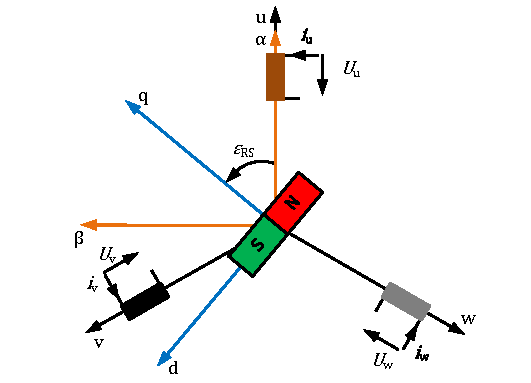
\includegraphics[width=0.8\textwidth]{img/synchron-grundlage}
\caption{Graphische Veranschaulichung der verschiedenen Koordinatensysteme, ständerfest $(\alpha, \beta)$ und rotorfest $(d, q)$.}
\label{fig:synchron-grundlage}
\end{figure}
\end{frame}

\subsection{Linearisierte Gleichungen}
\begin{frame}{Linearisierte Gleichungen}
\begin{itemize}
\pause \item Definitionsgemäß sind keine Sättigungserscheinungen vorhanden \autocites{mullerII2008}{schroder2001}
\pause \item Alle elektrischen Parameter einer PMSM und damit auch die Induktivitäten sind konstant
\end{itemize}

%\pause{\begin{align}
%\Psi_\x{d} &= \Psi_\x{pm} + L_\x{d} i_\x{d} \label{eqn:psid}\\
%\Psi_\x{q} &= L_\x{q} i_\x{q} \label{eqn:psiq} \\
%M_\x{i} &= \frac{3p}{2}(\Psi_\x{d} i_\x{q} - \Psi_\x{q} i_\x{d}) %\label{drehmoment}
%\end{align}

%(vgl.~\textcite{schroder2001})}
\end{frame}

\begin{frame}{Linearisierte Gleichungen}\label{fol:lin-gleichungen}
\begin{block}{Spannungsgleichungen des linearisierten Modells}
\begin{align}
u_\x{d} &= R_\x{1} i_\x{d} + L_\x{d} \frac{\x{d}i_\x{d}}{\x{d}t} - \omega_\x{el}L_\x{q} i_\x{q}  \label{uq-allg} \\ 
u_\x{q} &= R_\x{1} i_\x{q} + L_\x{q} \frac{\x{d}i_\x{q}}{\x{d}t} + \omega_\x{el}L_\x{d} i_\x{d} + \omega_\x{el}\Psi_\x{pm} \label{ud-allg} \\ 
M_\x{i} &= \frac{3p}{2}(\Psi_\x{pm} i_\x{q} + (L_\x{d} - L_\x{q})i_\x{d} i_\x{q})
\end{align}
(vgl.~\textcite{schroder2001})
\end{block}
\end{frame}

\begin{frame}[plain]{Linearisierte Gleichungen}
\begin{figure}[!t]
\centering
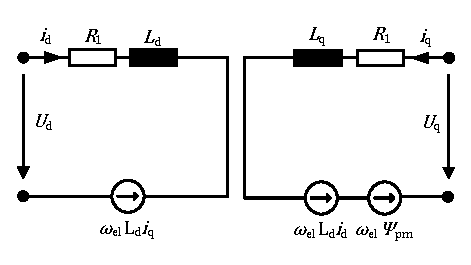
\includegraphics[width=\textwidth]{img/spannungsgleichungen}
\caption{Graphische Darstellung der Gleichungen Gl.~(\ref{uq-allg}) und Gl.~(\ref{ud-allg}).}
\label{fig:spannungsgleichungen}
\end{figure}
\end{frame}

\subsection{Allgemeine Gleichungen}
\begin{frame}{Allgemeine Gleichungen}
\begin{itemize}
\pause \item Induktivitäten ändern sich $\rightarrow$ abhängigkeit: Belastung
\pause \item Grund: Sättigungseffekte, Kreuzkopplung~--~entsteht durch Beeinflussung der verkoppelten Induktivitäten
\pause \item z.\ B.\ in der realen Maschine verlaufen die Ströme $i_\x{d}$ und $i_\x{q}$ in dem gleichen Ständerblech \autocite{Kellner2012}
\pause \item Bei Verwendung der linearen Gleichungen (s.~h.~Folie~\ref{fol:lin-gleichungen}) werden Sättigungseffekte vernachlässigt
\pause \item Unter Berücksichtigung der Eisenverluste bzw. Wirbelstromverluste reichen die Gleichungen nicht mehr aus
\end{itemize}
\end{frame}

\begin{frame}{Neue Gleichungen für $\Psi_\x{d}$ und $\Psi_\x{q}$}\label{fol:allg-flussverkettung}
\begin{itemize}
\pause \item Einige Ansätze unterteilen die Induktivitäten in Selbst- und Gegeninduktivitäten \autocite{stumberger_evaluation_2003}
\pause \item Dabei sind sowohl die Selbst- als auch die Gegeninduktivität jeweils von den Strömen abhängig $\rightarrow$ Hysterese
\end{itemize}

\pause{\begin{align}
\Psi_\x{d} &= \Psi_\x{pm} + L_\x{dd}^{\xi}(i_\x{d})\cdot i_\x{d} + L_\x{dq}^{\xi}(i_\x{d} ,i_\x{q})\cdot i_\x{q} \\
\Psi_\x{q} &= L_\x{qq}^{\xi}(i_\x{q})\cdot i_\x{q} + L_\x{qd}^{\xi}(i_\x{d} ,i_\x{q})\cdot i_\x{d}
\end{align}

(vgl.~\textcite{stumberger_evaluation_2003})}

\end{frame}

\begin{frame}{Darstellungsweise der Induktivitäten}\label{fol:darstellung-induktiv}
\pause Nach \textcite{Kellner2012} ist es möglich die Induktivitäten intuitiv darzustellen als:

\pause{\begin{align}
L_\x{d}^{(i_\x{d},i_\x{q})} &= L_\x{dd}^{\xi}(i_\x{d}) + L_\x{dq}^{\xi}(i_\x{d},i_\x{q})\cdot\frac{i_\x{q}}{i_\x{d}} \\
L_\x{q}^{(i_\x{d},i_\x{q})} &= L_\x{qq}^{\xi}(i_\x{q}) + L_\x{qd}^{\xi}(i_\x{d},i_\x{q})\cdot\frac{i_\x{d}}{i_\x{q}}
\end{align}}

\pause $\rightarrow$ Mehrwert wegen Trennung der Selbst- und Gegeninduktivität?

\end{frame}

\begin{frame}
\pause Anhand Folie~\ref{fol:darstellung-induktiv} lassen sich damit die Flussverkettung von Folie~\ref{fol:allg-flussverkettung} vereinfachen:
\vspace*{0.5cm}
\pause{\begin{block}{Flussverkettungen der allgemeinen Maschinengleichungen}
\begin{align}
\Psi_\x{d}^{(i_\x{d},i_\x{q})} &= \Psi_\x{pm}^{(i_\x{d},i_\x{q})} + L_\x{d}^{(i_\x{d},i_\x{q})}\cdot i_\x{d} \\
\Psi_\x{q}^{(i_\x{d},i_\x{q})} &= L_\x{q}^{(i_\x{d},i_\x{q})}\cdot i_\x{q}
\end{align}
Diese Darstellungsweise ist kürzer und übersichtlicher
\end{block}}
\end{frame}

\begin{frame}{Allgemeine Maschinengleichungen in Zustandsform}

\begin{align}
\left( \begin{array}{c} u_\x{d} \\ u_\x{q} \end{array} \right) &= \left( \begin{array}{cc} R_\x{1} & -\omega_\x{el}L_\x{q}^{(i_\x{d},i_\x{q})} \\ \omega_\x{el}L_\x{d}^{(i_\x{d},i_\x{q})} & R_\x{1} \end{array} \right) \left(\begin{array}{c} i_\x{d} \\ i_\x{q} \end{array}\right) \label{eqn:allg-spannungsgleichung} \\ 
 &\ldots + \underbrace{\left( \begin{array}{cc} L_\x{dd}^{(i_\x{d},i_\x{q})} & L_\x{dq}^{(i_\x{d},i_\x{q})} \\ L_\x{qd}^{(i_\x{d},i_\x{q})} & L_\x{qq}^{(i_\x{d},i_\x{q})} \end{array}\right)}_{\text{differentielle Induktivitäten}} \dot{\left(\begin{array}{c} i_\x{d} \\ i_\x{q} \end{array} \right)} \nonumber \\ 
& \ldots + \left( \begin{array}{c} \frac{\x{\partial}}{\x{\partial }t} \Psi_\x{pm}^{(i_\x{q})} \\ \omega_\x{el} \Psi_\x{pm}^{(i_\x{q})} \nonumber \end{array}  \right) \nonumber
\end{align}
in Anlehnung an \autocite{Kellner2012}.
\end{frame}

\begin{frame}[plain]{Spannungsgleichungen der allgemeinen Maschinengleichungen}
\begin{figure}[!h]
\centering
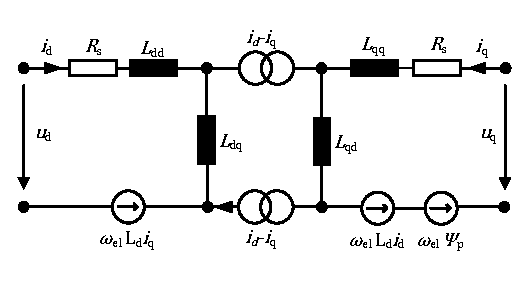
\includegraphics[width=\textwidth]{img/allg-spannungsgleichung}
\caption{Graphische Darstellung der Gleichungen (Gl.~\ref{eqn:allg-spannungsgleichung}).}
\label{fig:allg-spannungsgleichung}
\end{figure}
\end{frame}

\section{Ansätze zur Identifikation}
\subsection{Bestimmung der Rotorlage}
\begin{frame}{Bestimmung der Rotorlage}
	\begin{itemize}
		\item Geberlosen Regelung: Keinen Wartungsaufwand, geringere Kosten $\rightarrow$ keine Rotorposition bei niedrigen Drehzahlen? (Prinzip: Blockkommutierung durch das zurückmessen der im Motor induzierten Gegenspannung)
		\item Resolvers: Absolutwert der Rotorposition $\rightarrow$ Wartungsaufwand und höhere Kosten
		\item Inkrementalgeber: ist nicht sinnvoll, zu ungenau.
	\end{itemize}
\end{frame}

\begin{frame}[plain]{Überblick}
	\begin{figure}
		\begin{minipage}{0.3\textwidth}
			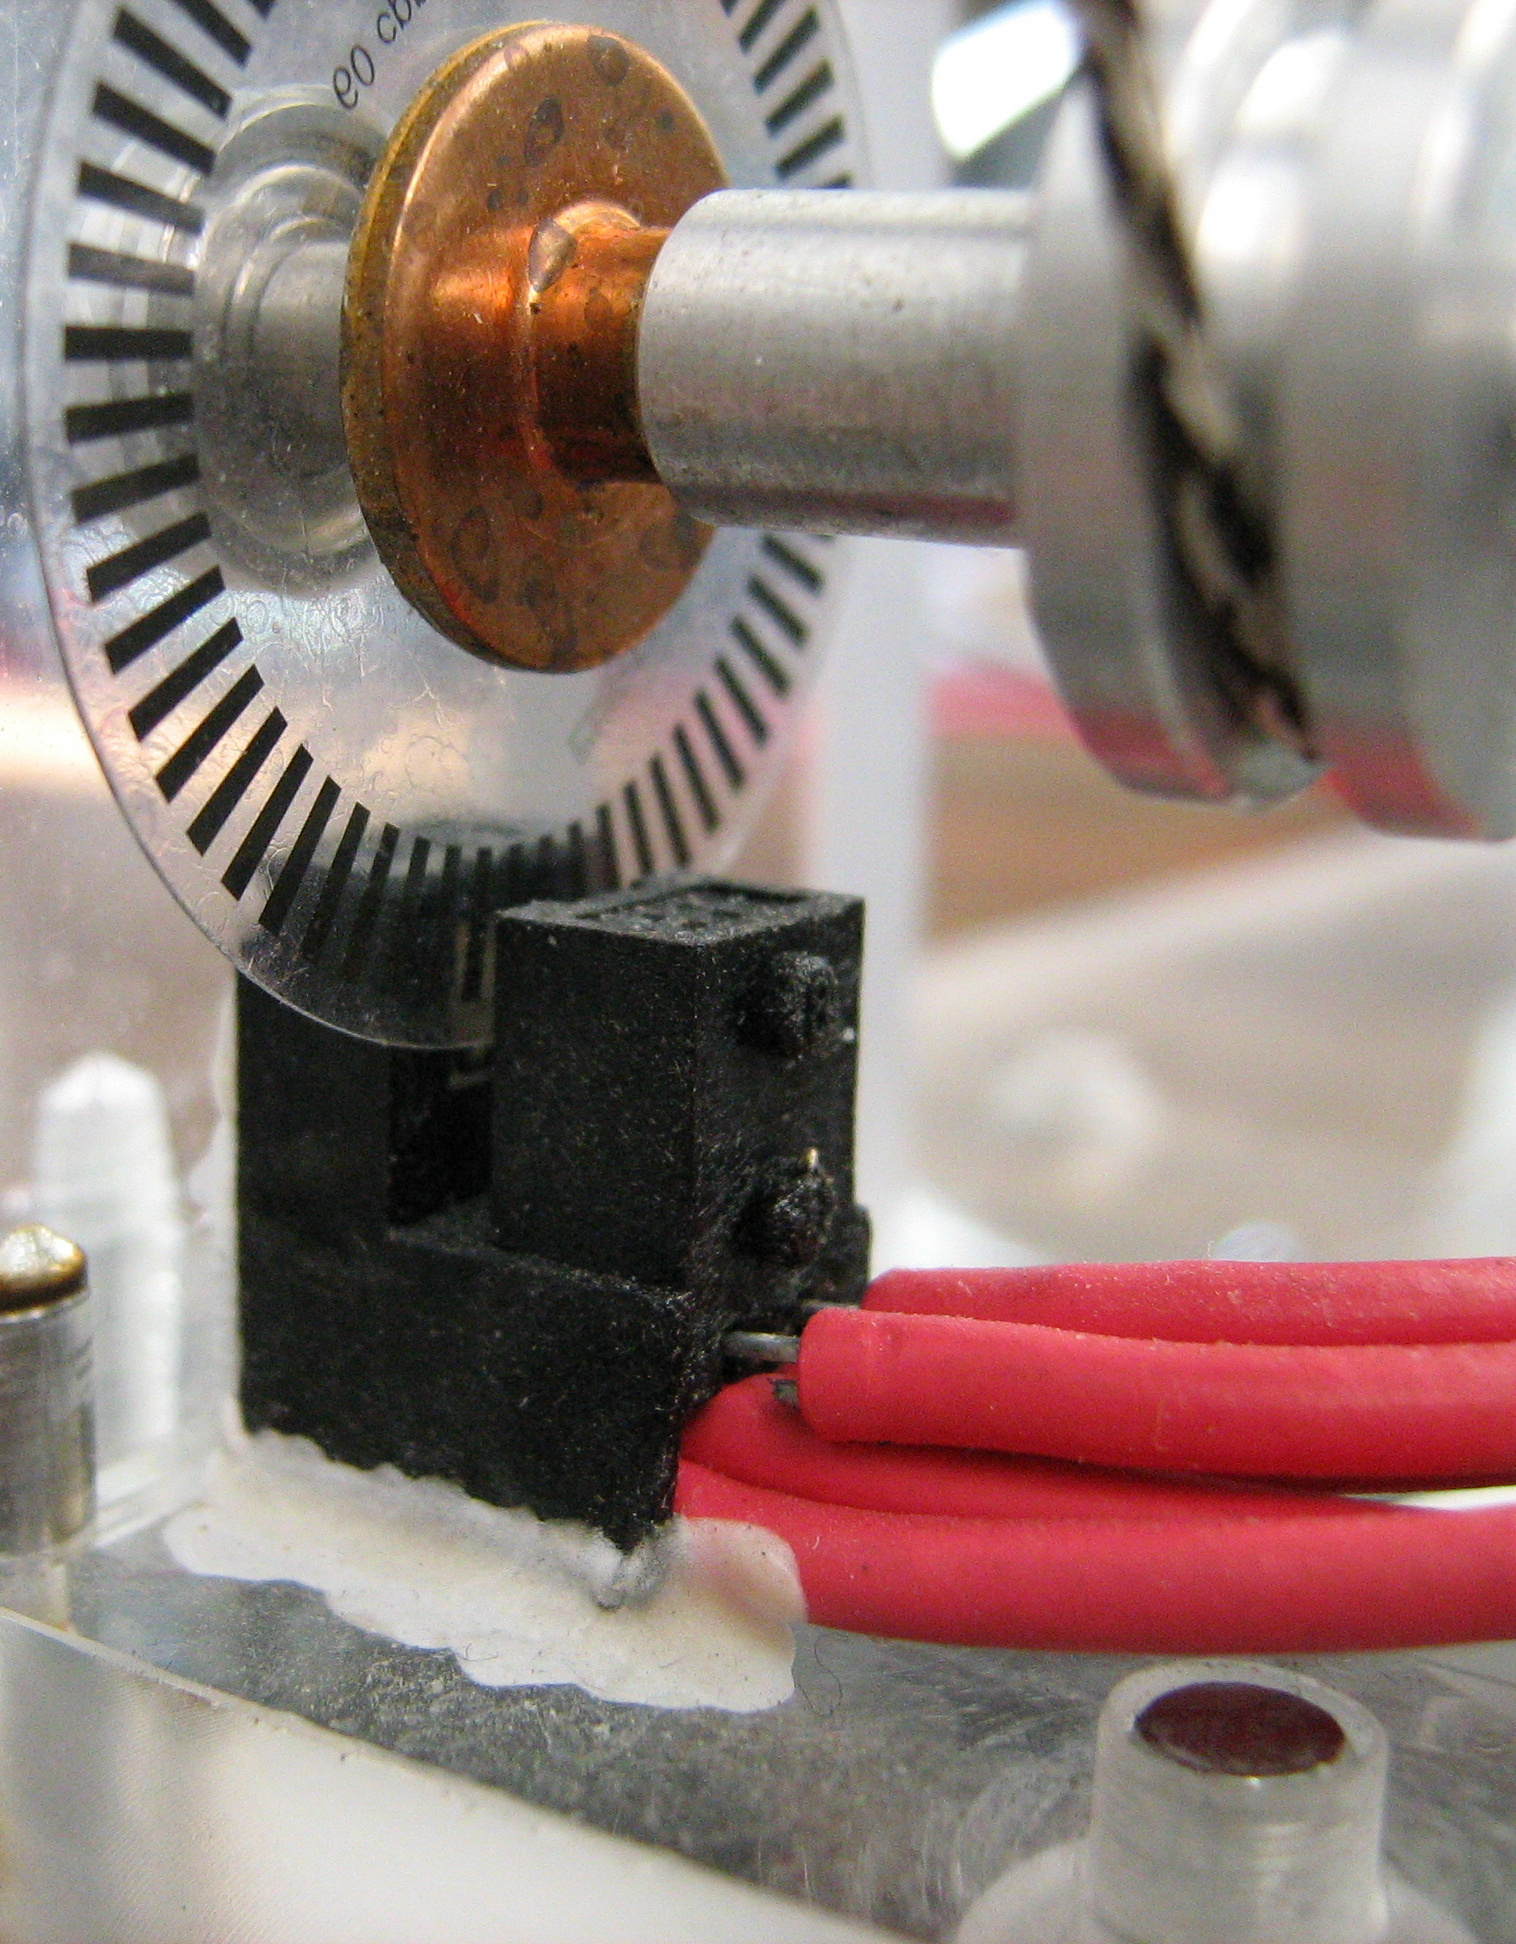
\includegraphics[width=\linewidth]{img/inkrementalgeber}
		\end{minipage}
		\begin{minipage}{0.3\textwidth}
			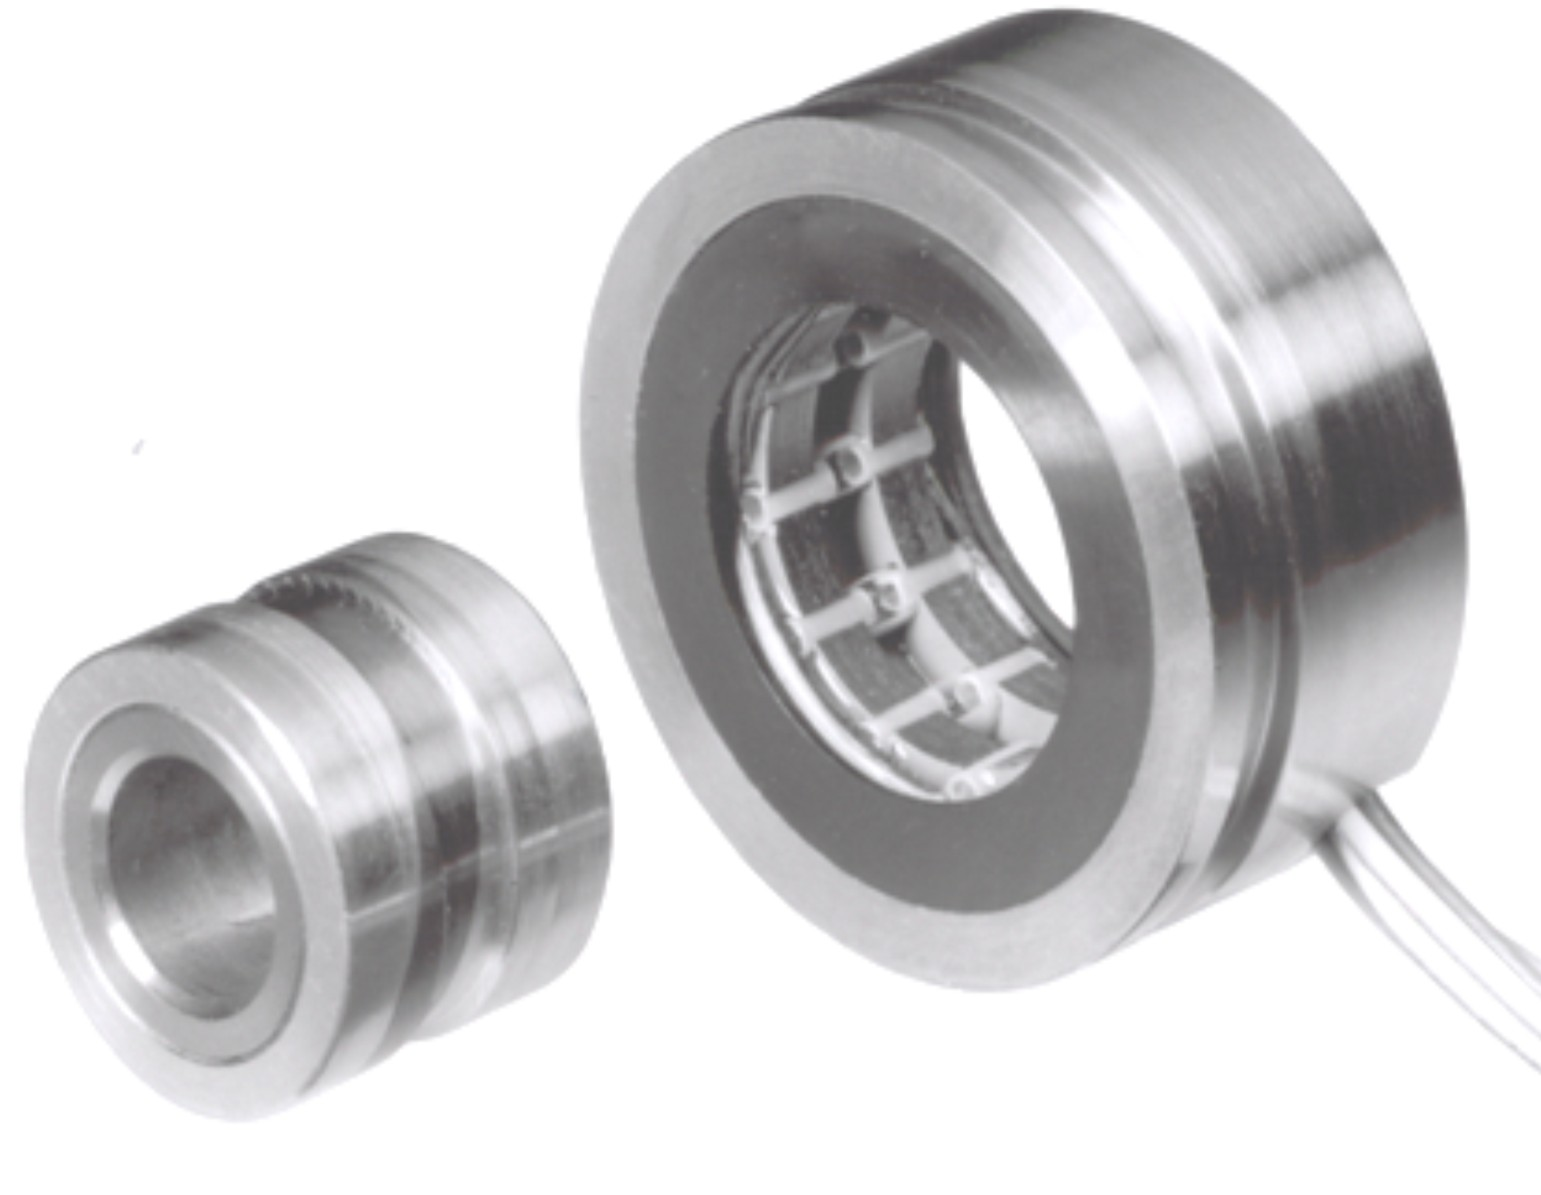
\includegraphics[width=\linewidth]{img/resolver.jpg}
		\end{minipage}
		\begin{minipage}{0.3\textwidth}
			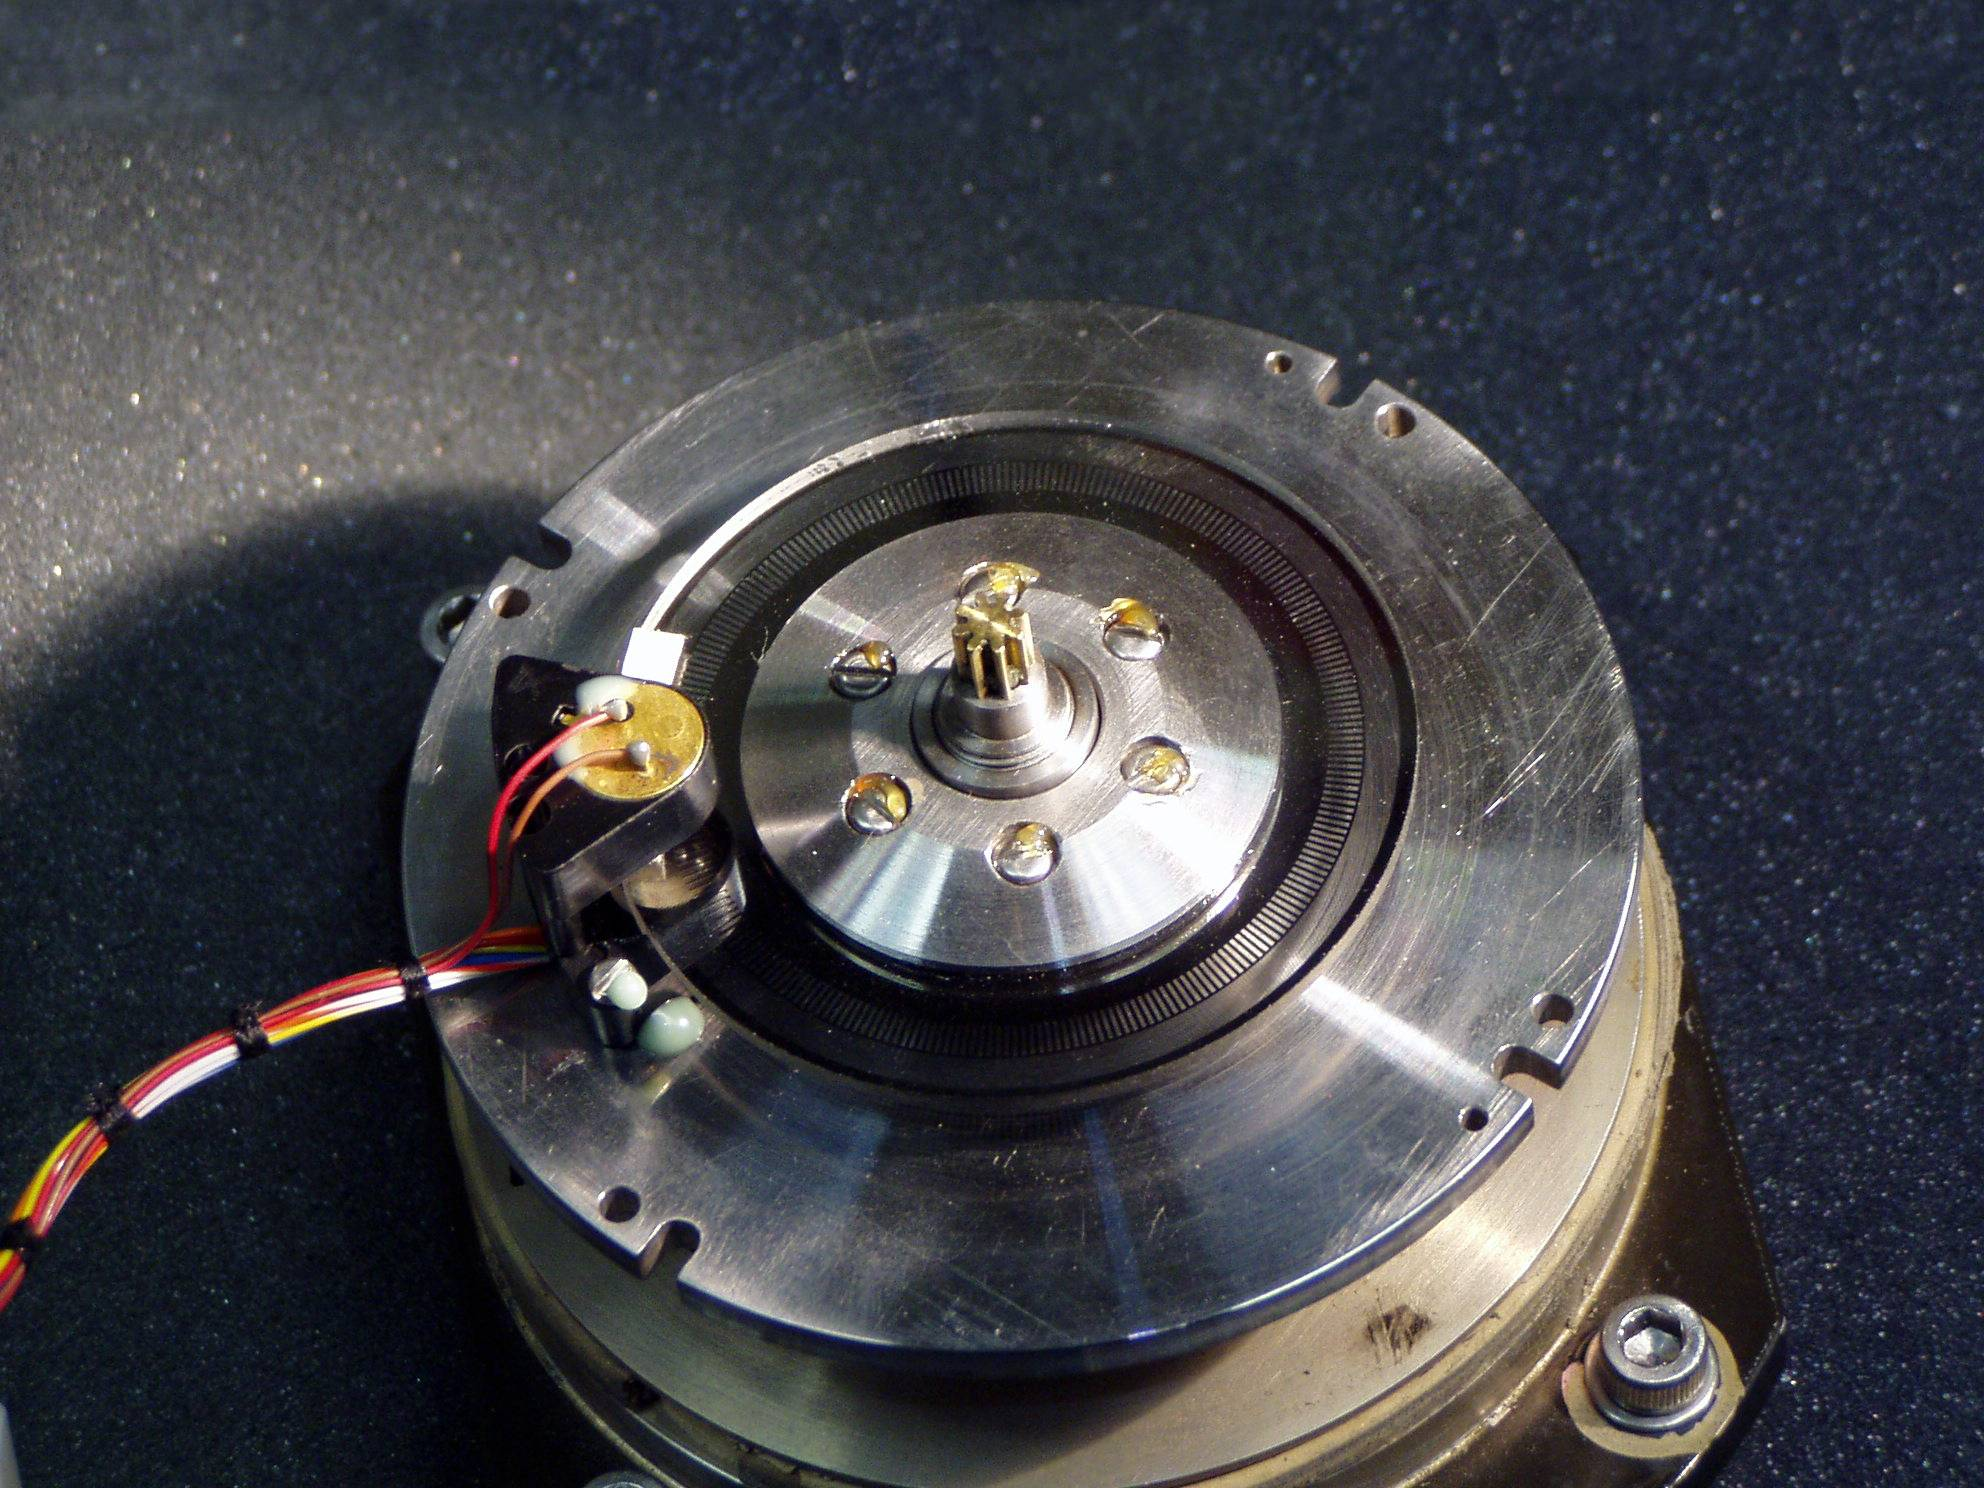
\includegraphics[width=\linewidth]{img/encoder}
		\end{minipage}
		\caption{Links: Inkrementalgeber mit Gabellichtschranke, Autor: Tycho. Mitte: Resolver, Quelle: MICRONOR~--~Hollow Shaft Standard Resolver, Size 15: RE3616 . x. Rechts: Optischer Encoder, 16834 Impulse pro Umdrehung. Autor: Charly Whisky.}
	\end{figure}
\end{frame}

\begin{frame}{Geberlose Regelung}
	\begin{itemize}
		\item Testsignalverfahren für niedrige Drehzahlen
		\item Differentieller Schenkligkeitskoeffizient
		\item EMK-Verfahren für hohe Drehzahlen
	\end{itemize}
\end{frame}

\subsection{Identifikation der Induktivitäten und des Ständerwiderstandes}

\begin{frame}{Online Identifikation?}
	\begin{itemize}
		\item Ansätze dazu in \autocite{underwood_online_2010}
		\item Zweifelhafte Stabilität und Genauigkeit in \autocite{underwood_online_2010}
		\item $\rightarrow$ Bisherige Online Messverfahren gelangen an ihre Grenze, die Notwendigkeit wird in Frage gestellt:
	\end{itemize}
	
	\begin{quote}
		\enquote{Zum einen ändern sich die Induktivitäten im Wesentlichen nur abhängig von den Strömen $i_\x{d}$ und $i_\x{q}$, kaum aufgrund von anderen äußeren Umgebungseinflüssen beziehungsweise Prüfstandsparametern, wie zum Beispiel Temperatur oder Drehzahl des Systems \autocite[S.~79]{Kellner2012}.}
	\end{quote}
	
\end{frame}

\begin{frame}[plain]{Absolute und differentielle Induktivitäten}
	\begin{figure}[!h]
		\centering
		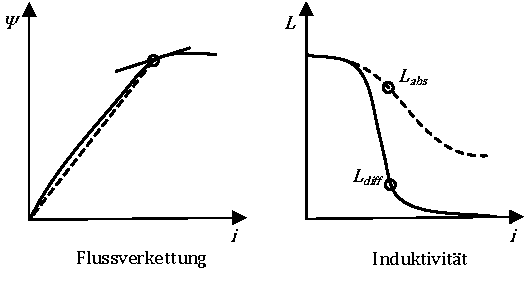
\includegraphics[width=\columnwidth]{img/induktiv}
		\caption{Prinzipielle Darstellung der Beziehung zwischen absoluter und differentieller Induktivität in Anlehnung an \textcite[S.~2]{kellner_general_2011}.}
		\label{fig:induktiv}
	\end{figure}
\end{frame}

\begin{frame}[plain]{Absolute Induktivitäten}
Theorie zur Messung der absoluten Induktivitäten
\begin{itemize}
	\item Für eine konstante Drehzahl wird ein $(i_\x{d},i_\x{q})$-Strompaar eingeprägt
	\item Für diesen Zustand werden die $d,q$-Spannungen und die Drehzahl gemessen
	\item Daraus lassen sich die Induktivitäten $L_\x{d}^{(i_\x{d},i_\x{q})}$ und $L_\x{q}^{(i_\x{d},i_\x{q})}$ berechnen
\end{itemize}
\begin{align}
	L_\x{d}^{(i_\x{d},i_\x{q})}  &= \frac{\Psi_\x{d}^{(i_\x{d},i_\x{q})}-\Psi_\x{d}^{(i_\x{d}=0,i_\x{q})}}{i_\x{d}} \\
	L_\x{q}^{(i_\x{d},i_\x{q})}  &= \frac{\Psi_\x{q}^{(i_\x{d},i_\x{q})}-\Psi_\x{q}^{(i_\x{d},i_\x{q}=0)}}{i_\x{q}}
\end{align}
(vgl.~\textcite{Kellner2012})
\end{frame}

\begin{frame}{Identifikation in der Praxis}
\begin{enumerate}
	\item Jede Kombination aus $i_\x{d}$- und $i_\x{q}$-Strömen; Lastmaschine muss einen const.\ Drehzahlsollwert realisieren können
	\item Konstante mittlere Drehzahl
	\item Über den Messbereich werden einzelne Betriebspunkte eingestellt
	\item Stationärer Zustand $\rightarrow$ Messwerte werden gespeichert
	\item Induktivitäten werden gemäß Gleichungen berechnet
\end{enumerate}
\end{frame}

\begin{frame}{Differentielle Induktivitäten}
\begin{itemize}
	\item Nur notwendig, wenn Stromänderung vorhanden (dynamische Vorgänge)
\end{itemize}

Theorie zur Messung von differentiellen Induktivitäten

\begin{itemize}
	\item Überlagerung mit einem hochfrequenten Signal
	\item Zu den stationären Arbeitspunkten wird ein hochfrequentes Testsignal addiert
	\item Aus der hochfrequenten Sprungantwort lässt sich die differentielle Induktivität berechnen
\end{itemize}
\end{frame}

\begin{frame}{Identifikation in der Praxis}
\begin{enumerate}
	\item Bestimmung des Ständerwiderstandes
	\item Einstellen der Strompaare
	\item Einprägung eines Testsignals mit einer vorgegebenen Frequenz in $q$-Richtung
	\item $\rightarrow (L_\x{qq},L_\x{dq})$
	\item Einprägung eines Testsignals mit einer vorgegebenen Frequenz in $d$-Richtung
	\item $\rightarrow (L_\x{dd},L_\x{qd})$
\end{enumerate}
\end{frame}

\begin{frame}{Ständerwiderstand und -temperatur}
Viele Autoren verwenden MRAC-Algorithmen \enquote{(model-reference adaptive control)} zur Identifikation des Ständerwiderstandes
\end{frame}

\begin{frame}[plain]{MRAC-Alrogrithmus}
\begin{figure}[h!]
	\centering
	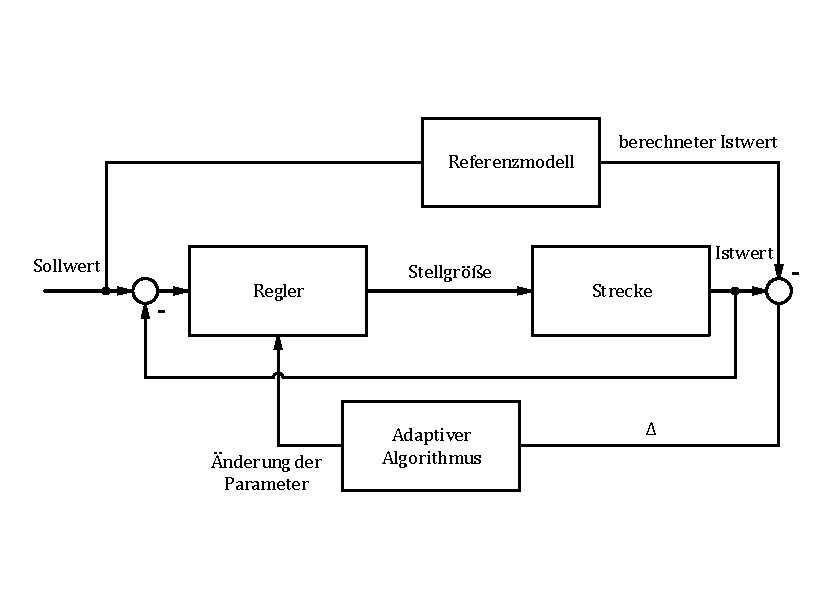
\includegraphics[width=\columnwidth]{img/mrac}
	\caption{Prinzipielle Darstellung eines MRAC-Systems in Anlehnung an \textcite{slotine_applied_1991}.}
	\label{fig:mrac}
\end{figure}
\end{frame}

\begin{frame}{Ständerwiderstand und -temperatur}
\begin{quote}
\enquote{Wenn die Parameter der PMSM nicht genau bekannt sind, dann ist es auch nicht möglich, ein genaues Referenzmodell der Maschine zu erstellen, weil dieses ja in irgendeiner Weise die Parameter enthalten müsste. \autocite[S.~139]{Kellner2012}}
\end{quote}
\end{frame}

\begin{frame}{Konventioneller Ansatz~--~$u_\x{d}$-Spannungsgleichung}
\begin{itemize}
	\item Auswertung der $u_\x{d}$-Spannungsgleichung
	\item $\rightarrow$ so beschreibt die $u_\x{d}$-Spannungsgleichung das Modell für ideal bekannte Parameter
	\item $u_\x{d}$ wird von der feldorientierten Regelung als Grundlage für den Spannungsraumzeiger ausgegeben
\pause	\item $\rightarrow$ unpraktisch da, ein feldschwächender Strom vorhanden sein muss, um die Widerstandsdifferenz zu berechnen \autocite{Kellner2012}
\pause 	\item $\rightarrow$ Energetische Gründe, prinzipiell möglich
\end{itemize}
\end{frame}

\begin{frame}{Identifikation mit Testsignalen}
	\begin{itemize}
		\item Einprägung von niederfrequenten $i_\x{d}$-Strom-Testsignalen
		\item Unterschied: Art der Einprägung und Auswertung der Sprungantwort
	\end{itemize}
	
	\begin{quote}
		\enquote{Das entwickelte Verfahren beruht auf der Annahme, dass die relevanten Störungen der Messsignale zum Teil Gleichtaktstörungen beziehungsweise Offsetfehler sind \autocite[S.~148]{Kellner2012}.}
	\end{quote}
	
\end{frame}

\begin{frame}{Ständertemperatur}
	\begin{itemize}
		\item Hängt immer mit der Identifikation des Ständerwiderstandes zusammen
		\item Ständerwiderstand bekannt $\rightarrow$ Temperatur bekannt
	\end{itemize}
	
		\begin{quote}
			\enquote{Die Ansätze in der Literatur zeigen, dass der an sich oft selbst gestellte Anspruch an die Genauigkeit der Temperaturberechnung nur selten erreicht werden kann. \autocite[S.~175]{Kellner2012}.}
		\end{quote}
		
\begin{align}
R_\x{1} = R_\x{1,ref} \cdot (1 + \alpha_\x{Cu}(\vartheta_\x{1}-\vartheta_\x{ref}))
\end{align}
	
\end{frame}



\section{Parameterfehler}
\begin{frame}
\begin{itemize}
	\item Je größer der Fehler, desto weniger bilden die Modelle die Realität ab
	\item Die Parameter $R_\x{1}, L_\x{d,q}$ und $\Psi_\x{pm}$ können nicht direkt gemessen werden
	\item Fehlerforpflanzung
	\item Probleme bei der \enquote{geberlosen Regelung}
	\item Fehler: Messgrößen sind Ungenauigkeiten der Umrichterlinearisierung oder Toleranzen der Stromsensoren
\end{itemize}
\end{frame}

\section*{Bibliography}
\begin{frame}[allowframebreaks]{Bibliography}
\nocite{ternesfeldkamp}
\nocite{Bruhn2009}
\nocite{Perassi2006}
\nocite{genduso}
\nocite{fischer2009}
\printbibliography
\end{frame}

\begin{frame}[plain]{Vielen Dank für Ihre Aufmerksamkeit}	
	\huge{Fragen?}		
\end{frame}

%\section*{Anhang}


\end{document}